%%%%%%%%%%%%%%%%%%%%%%%%%%%%%%%%%%%%%%%%%%%%%%%%%%%%%%%%%%%%%%%%%%%%%%%%%%%%%%%%
%2345678901234567890123456789012345678901234567890123456789012345678901234567890
%        1         2         3         4         5         6         7         8

\documentclass[letterpaper, 11 pt, conference]{ieeeconf}  % Comment this line out if you need a4paper

%\documentclass[a4paper, 10pt, conference]{ieeeconf}      % Use this line for a4 paper

\IEEEoverridecommandlockouts                             %https://www.overleaf.com/2156968253fhhpgmhwnfrt % This command is only needed if 
                                                          % you want to use the \thanks command

\overrideIEEEmargins                                      % Needed to meet printer requirements.

%In case you encounter the following error:
%Error 1010 The PDF file may be corrupt (unable to open PDF file) OR
%Error 1000 An error occurred while parsing a contents stream. Unable to analyze the PDF file.
%This is a known problem with pdfLaTeX conversion filter. The file cannot be opened with acrobat reader
%Please use one of the alternatives below to circumvent this error by uncommenting one or the other
%\pdfobjcompresslevel=0
%\pdfminorversion=4

% See the \addtolength command later in the file to balance the column lengths
% on the last page of the document

% The following packages can be found on http:\\www.ctan.org
\usepackage{graphics} % for pdf, bitmapped graphics files
\usepackage{epsfig} % for postscript graphics files
\usepackage{mathptmx} % assumes new font selection scheme installed
\usepackage{times} % assumes new font selection scheme installed
\usepackage{amsmath} % assumes amsmath package installed
\usepackage{amssymb}  % assumes amsmath package installed
\usepackage{graphicx}
\usepackage{subcaption}
\usepackage{multirow}
\usepackage{booktabs}
\usepackage{comment} % for comment command
\usepackage{soul, color} % for hl command
\usepackage{hyperref}

\title{\huge \bf Fraud Detection - A Machine Learning Perspective}
\author{Vibhavasu Pasumarti - EP20BTECH11015\footnote{\href{emailto:ep20btech11015@iith.ac.in}{ep20btech11015@iith.ac.in}}}


%\author{ <-this % stops a space
% \thanks{}% <-this % stops a space
% \thanks{$^{1}$ Undergraduate Student, Electrical Engineering, IIT Hyderabad
%         {\tt\small ee15btech11030@iith.ac.in}}%
% \thanks{$^{2}$Undergraduate Student, Electrical Engineering, IIT Hyderabad
%         {\tt\small ee15btech11006@iith.ac.in}}%
% \thanks{$^{3}$Associate Professor, Electrical Engineering, IIT Hyderabad
%         {\tt\small ee15btech11006@iith.ac.in}}%
%}

\renewcommand{\thefootnote}{\roman{footnote}}

\begin{document}
\maketitle

\begin{abstract}
    In this work, I explore how various classification algorithms detect genuine or fraudulent transactions in a dataset containing transactions done in September 2013 in Europe. The dataset, derived from PCA transformation, contains numerical features, with "Time elapsed between two transactions" and "Amount" preserved. The challenge lies in imbalanced dataset, with more real transactions than fraudulent ones. Different classifiers are tested to see how they handle this imbalance. Subsequently, various imbalance handling algorithms will be applied, and their effects on the results will be observed.
\end{abstract}

\section{Introduction}\label{sec:intro}
Credit card fraud is a big problem today. Quickly detecting fraudulent transactions might give a better chance of recovery.

\subsection*{Dataset}
\begin{itemize}
\item[-] The dataset obtained from Kaggle contains 284,807 transactions done in Europe during September 2013, out of which 492 have been marked fraudulent. Each transaction is marked whether fraudulent or not.
\item[-] The dataset contains 30 features, of which 28 features have been obtained from PCA transformation of original features.
\item[-] This has been done to preserve confidentiality.
\item[-] However, ``Time elapsed between two transactions" and ``Transaction Amount" are presented as such and have not been treated with the former method.
\end{itemize}

However, the dataset is highly skewed. The no.of normal transactions significantly outnumber the no.of positive transactions. For the preliminary run, the dataset is split into training, and testing sets in the ratio (70:30). For the final run, split into training, validation and testing sets in the ratio (70:15:15)

\section{Objective}
Explore how different Machine Learning algorithms work to classify the transactions in the given dataset as legitimate or fraudulent.
% \vspace{\fill}

In an ML perspective, this represents a \emph{Classification} problem.

\section*{Algorithms employed}
% \subsubsection{Classifiers}
\noindent For this project, the following classification algorithms are used:
\begin{itemize}
    \item k - Nearest Neighbours Classifier
    \item SVM (Support Vector Machine) + soft margin
    \item Logistic Regression Classifier
    \item Na\"ive Bayes Classifier%\footnote{Will be shown in the final report\label{futnote}}
    \item Decision Trees%\footref{futnote}
    \item Neural Networks%\footref{futnote}
    % \item 
\end{itemize}
The following metrics will be used to compare the results. 
\begin{itemize}
    \item F1 - Score
    \item Log loss
    \item Recall/True Positive Rate
	\item Negative Predictive Value\footnote{\tiny Not displayed for other classifiers as final report is instructed to be an \textit{extension} to the intermediate report\label{key}}
    \item True Negative Rate\footref{key}
    \item False Negative Rate\footref{key}
    \item False Discovery Rate\footref{key}

    \item Precision/Positive Predictive Value$^**$
\end{itemize}
% \subsubsection{Imbalance Handlers}
% The following methods are used
% \begin{itemize}
%     \item SMOTE
%     \item Re-sampling (Oversampling and Undersampling)
%     \item Boosting
%     \item Bagging
    
% \end{itemize}
% \section{Methods}\label{sec:methods}

\section{Preliminary Results}\label{sec:result}
% \subsection{Preliminary run}
The dataset is classified using \textit{vanilla} SVM, k-NN, and Logistic Regression classifiers in this run.

\subsection{Confusion Matrices}
% \begin{itemize}
% \noindent- Soft margin SVM classifier: C = 15\\
% - k-NN classifier: k = 5
% \end{itemize}

\begin{figure}[h]
    \centering
    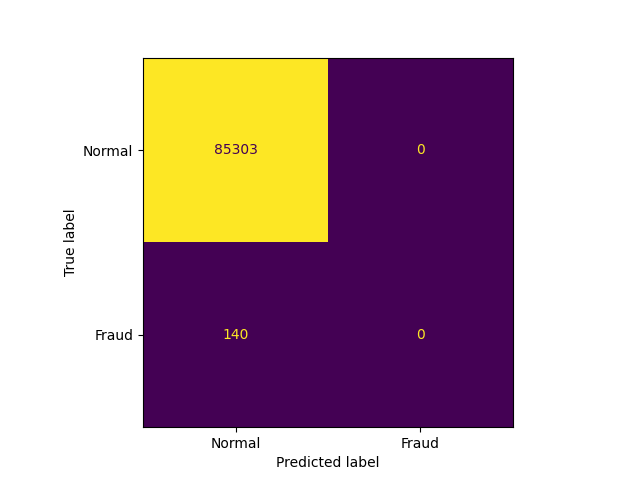
\includegraphics[width=0.92\columnwidth]{Images/SVM_CF.png}
    \caption{Support Vector Classifier; C = 15}
    \label{fig:SVC_CF}
\end{figure}
\begin{figure}[h]
    \centering
    \includegraphics[width=\columnwidth]{Images/kNN_CF.png}
    \caption{k-NN Classifier}
    \label{fig:knn_CF}
\end{figure}
\begin{figure}[h]
    \centering
    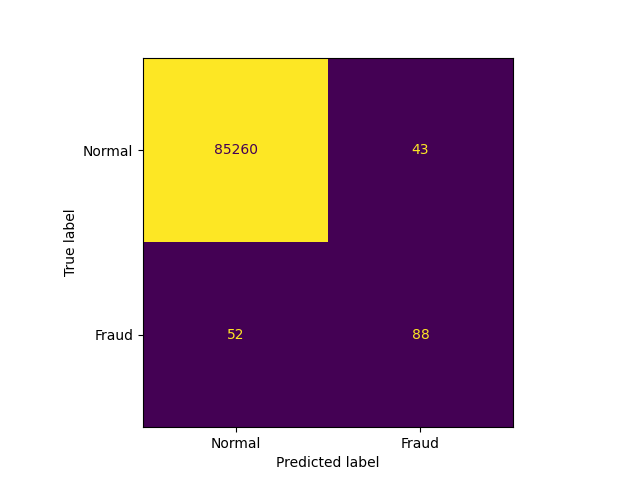
\includegraphics[width=\columnwidth]{Images/LogR_norm_CF.png}
    \caption{Logistic Regression Classifier}
    \label{fig:LogR_CF}
\end{figure}

\vspace{5em}

\subsection{Discussion}
\noindent\textbf{Observation:} From the confusion matrces of SVM Fig:\ref{fig:SVC_CF} and kNN Fig:\ref{fig:knn_CF}, we see that most transactions are predicted as \textit{normal}. \\
\textit{Accuracy} is a bad metric as the number of FN is almost equal to the total no.of datapoints. This is because of the unbalanced nature of the dataset as discussed in \ref{sec:intro}.\\
\textit{Precision} is not useful because it does not depend on True Negatives or False Negatives, and our aim is to detect fraudulent or True Negatives. It will be used as the last criterion while selecting a classifer.\\
The metrics (in table \ref{tab:metric1}) such as \textit{F1-Score} and, \textit{Recall} are very low, but they are moderately good for Logistic regression Fig:\ref{fig:LogR_CF}. \\\vspace{5em}

\begin{table}[h]
    \centering
    \begin{tabular}{|l|c|c|c|c|}
    \hline
         Model &  Precision & Recall & F1 Score & Log loss
         \\\hline
         SVM & 0 & 0 & 0 & 0.059 \\
         k-NN & 0.909 & 0.143 & 0.247 & 0.051\\
         Logistic regression & 0.672 & 0.629 & 0.649 & 0.040\\\hline
         
    \end{tabular}
    \caption{Metrics for SVM and k-NN}
    \label{tab:metric1}
\end{table}
% % \textbf{Reason:}
% % This is because different features have different ranges. So distance-based models like \textit{SVM} and \textit{kNN} would be biased towards features like \textit{Transaction amount}, which have a very high range.
% % \\
% % \textbf{How to resolve this?}\\
% % \textit{Normalize/Scale} all the features.

% % \subsection{After Normalization}
% % \begin{figure}[h]
% %     \centering   
% %     \includegraphics[width=\columnwidth]{Images/kNN_norm_CF.png}
% %     \caption{Scaled dataset +  k-NN Classifier}
% %     \label{fig:kNN_norm_CF}
% % \end{figure}

% \noindent\textbf{Observation:}
% Now, we see that the models are able to detect some of the fraudulent transactions.\\
% However, these models are able to detect \textit{less than} $10\%$ of all fraudulent transactions. But the metrics like recall $> 50 \%$ and precision $=1$. This shows how highly imbalanced datasets can disrupt the metrics

\textbf{Reason:}
This is because the data is highly imbalanced
\subsubsection{For SVM} The objective is 
\begin{multline}
% f(x) = sign(\sum_i \alpha_i \times y_i \times(K(x_i, x) + b)
% L_{p}=\frac{\|w\|^{2}}{2}+C \sum_{i=1}^{n} \xi_{i} \cr - \sum_{i=1}^{n} \alpha_{i}\left[y_{i}\left(w \cdot x_{i}+b\right) - 1+\xi_{i}\right] - \sum_{i=1}^{n} r_{i} \xi_{i}
\min(\|w\|^{2} + C \sum_{i=1}^{n} \xi_{i})\\ \text{ s.t. } y_i (w \cdot f(x_i) + b) \geq 1 - \xi_i \quad \text{where   } \xi_i \geq 0
\label{eq:SVM}
\end{multline}
% $K(x_i, x)$ is the Kernel function and $ 0 \leq \alpha_i \leq C$
% \section{Discussion}\label{sec:discussion}

The objective function has two parts: the first aims to maximize the separation between classes, while the second works to minimize mis-classifications. The parameter "C" is the cost assigned to mistakes, treating errors in both positive and negative cases equally.
In situations where one class significantly outnumbers the other, especially near the class boundary, the majority class (here: "normal"/negative class) tends to influence the decision boundary against the majority class. However, this shift can lead to more mistakes, and in extreme cases of imbalance, the model may even classify all points as belonging to the minority (here: "fraudulent/positive") class as "normal".~\cite{10.1007/978-3-540-30115-8_7}
\subsubsection{k-NN classifier}
decides the category of a new item by looking at the classes of its closest neighbors from the training data. However, in imbalanced datasets where some classes are larger than others, i.e, most of the nearest neighbours belong to the majority class. This makes kNN to favor the larger classes when making predictions.\\
\subsubsection{Logistic Regression Classifier} is robust to imbalanced datasets as it uses a function of negative log-likelihood (NLL $\cong$ MLE) as the loss function and gives probabilistic output. The NLL/MLE seeks parameters that maximize the likelihood of accurately predicting both majority and minority class instances, so the model remains balanced towards both classes. As the model outputs probabilities rather than discrete predictions, The logistic loss function used in logistic regression penalizes misclassifications proportionally, effectively handling imbalances in the data.\\
This also means that imbalance handling algorithms(\ref{sec:imbh}) do not increase the performance for Logistic Regression, as the maximum LLH looks to predict both positive and negative instances, so the no.of instances of each class do not create much bias.
\begin{figure}[h]
	\centering
	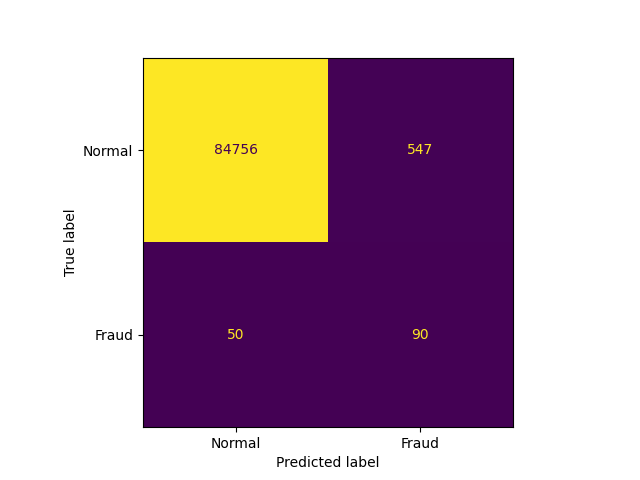
\includegraphics[width=0.92\columnwidth]{Images/GNB_norm_CF.png}
	\caption{Na\"ive Bayes Classifier}
	\label{fig:gnb_CF}
\end{figure}
\subsubsection{Na\"ive Bayes Classifier} is unfazed by data imbalance due to its underlying assumption of \textit{feature independence}. This assumption allows the classifier to estimate the class probabilities based on the individual feature probabilities, regardless of the class distribution.\\
Additionally, Na\"ive Bayes uses the maximum likelihood estimation to estimate the parameters of the feature probabilities. This estimation method is less affected by imbalanced datasets compared to other methods that rely on the overall class distribution\footnote{However, in an actual dataset, the assumption of independence does not hold, so the Na\"ive Bayes classifier cannot detect all the fraudulent transactions.}
\begin{figure}[h]
	\centering
	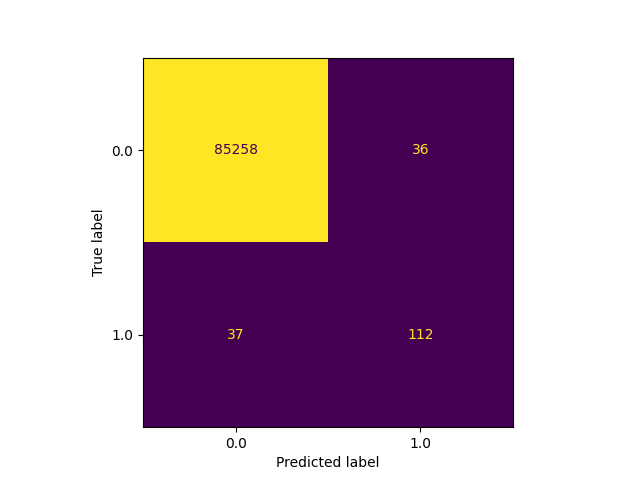
\includegraphics[width=0.92\columnwidth]{Images/dt_vanilla_CF.png}
	\caption{Decision Tree Classifier}
	\label{fig:dt_CF}
\end{figure}
\subsubsection{Decision Trees} is resistant to data imbalances as at each node, the because decision is taken based on the \textit{Gini} index. (or other impurity measures) which depend on \textit{proportions} rather than absolute counts. As a result, decision trees focus on the relative distribution of classes at each node, allowing them to be less sensitive to the absolute number of instances in each class.
\begin{center}
\begin{align*}
    \text{Gini index } G = \sum_c \Pi_c (1 - \Pi_c)
% \end{align*}
\intertext{where}
% \begin{align*}
    \Pi_c = \frac{\text{no.of points in the subspace with label } c}{\text{no.of points in the subspace}}
\end{align*}
\end{center}
Since these depend on \textit{proportions} rather than absolute counts decision trees focus on the relative distribution of classes at each node, allowing them to be less sensitive to the absolute number of instances in each class.

\begin{figure}[h]
	\centering
	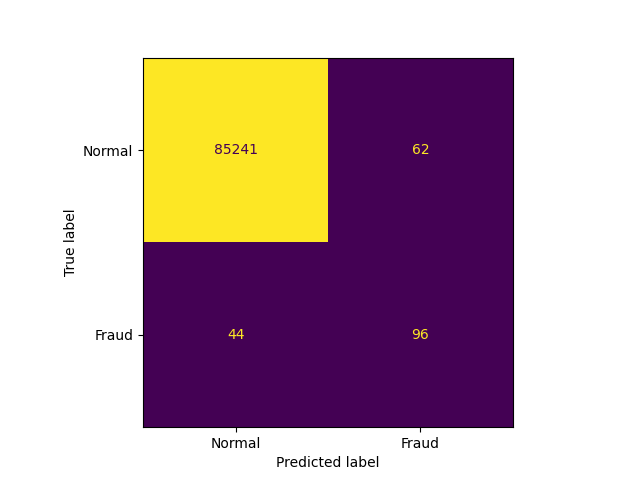
\includegraphics[width=0.92\columnwidth]{Images/MLP_norm_CF.png}
	\caption{Multi layer Perceptron}
	\label{fig:dt_CF}
\end{figure}

\subsubsection{Multi-Layer Perceptron/Neural Network}
In the training of an MLP, weights are updated using backpropagation and gradient descent. The weight updates are influenced by the gradient of the loss function with respect to the weights. In the case of imbalanced data, where one class has significantly fewer instances, the gradients associated with the minority class might be smaller. This can result in relatively smaller updates to the weights corresponding to the minority class during training. However, with higher dimensional MLPs, the overall prediction can be robust to imbalances as the number of nodes can counterbalance the small updates to the slow updation of weights.

\section{Results after imbalance handling}
\label{sec:imbh}
\subsection{Oversampling}
Oversampling\footnote{Random Oversampling} is a technique to combat data imbalance. In this method, instances from minority class are randomly selected with replacement. Then these newly sampled instances are added to the original dataset and this process is repeated again till the no.of instances in minority and majority class are (nearly) equal.
\subsection{SMOTE$^{\cite{SMOTE}}$}
SMOTE, or Synthetic Minority Oversampling Technique, is an oversampling method particularly useful when the quantity of data available for the minority class is insufficient.

SMOTE begins by randomly picking a data point from the minority class. It then identifies its neighbors. %The number of neighbors to consider is a parameter that can be adjusted.
A synthetic data point is then created at a random point between the chosen data point and one of its neighbors. This new point is not an exact copy of an existing data point, but rather a blend of two points, which helps to increase the diversity of the minority class in the dataset.

 The key advantage of SMOTE is that it creates synthetic, yet realistic, examples of the minority class, rather than simply duplicating existing instances, which can lead to overfitting. This makes the learning algorithm more effective as it has a richer, more diverse parts of the distribution to learn from.
\subsection{Undersampling}
Undersampling is a data imbalance handling technique used when one class has significantly more instances than another.

Instances in the majority class are randomly removed until it's size is approximately to the size of the minority class.

The result is a balanced dataset, with roughly equal numbers of instances for each class. A main drawback with this is that it can lead to the loss of information, as instances from the majority class are randomly removed.

\subsection{Bagging}%\footnote{For Compatible models only\label{fndt}}}
Bagging, short for Bootstrap Aggregating, is a technique used in machine learning to improve the stability and accuracy of prediction models. It's a type of ensemble learning method where multiple base models are trained independently and their predictions are combined to make the final prediction.

Here's a simplified explanation of how bagging works:

Bagging begins by creating multiple subsets of the original dataset using bootstrapping. Each subset is then used to train a separate base model. The base models are trained independently of each other, and they can be of any type (decision trees, logistic regression, etc.). Once all the base models are trained, they each make predictions on the same test data. The final prediction is made by aggregating the predictions from all the base models. The aggregation method depends on the type of problem. For regression problems, the average of the predictions is taken. For classification problems, the class that gets the most votes is chosen (also known as majority voting).

%The main advantage of bagging is that it reduces the variance of the prediction by introducing randomness into the model training process. This can help prevent overfitting, which is a common problem in machine learning where a model performs well on the training data but poorly on unseen data.
\subsection{Boosting\footref{fndt}}
Boosting is an ensemble method, which means it combines several "weak" models to create a "strong" model. The weak model is used to make predictions on the dataset, and the misclassified instances are identified. A new model is then trained, given more importance or \textit{weight} to the instances that were misclassified by the previous model. This process is repeated several times, with each new model focusing on the errors of the previous model. All the models are combined to make a final prediction. %Each model gets a say in the final prediction, but models that performed better have more influence.


\section{Choosing the best classifier for this data}
\begin{enumerate}
	\item The entire dataset is split into 3 parts: \textit{Train}, \textit{Validation} and \textit{Test}; in the ratio 0.7 : 0.15 : 0.15
	
	\item Each classifier is tested along with the above Imbalance handling techniques. The imbalance handling technique that shows the most performance is selected for that classifier.
	
	\item The (hyper-) parameters of each classifier are tuned using Grid Search Cross Validation using training and validation data.
	
	\item The \textit{Train} and \textit{Validation} data are combined each classifier with the optimized parameters along with the imbalance handling techniques, is trained on this combined dataset to create a final model.
	
	\item These final models are now tested on the \textit{untouched} test data and performance metrics of all models are used to determine which model suits the best for the given dataset.
\end{enumerate}

\begin{table}[h]
	\centering
	\begin{tabular}{|l|c|}
		\hline
		\textbf{Classifier} & \textbf{Chosen Technique}\\\hline
		SVM Classifier & Undersampling\\
		k-NN Classifier & Oversampling\\
		Logistic Regression Classifier & Bagging\\
		Na\"ive Bayes Classifier & Boosting\\
		Decision Trees & Bagging\\
		Multi-layer Perceptron & SMOTE	\\\hline
	\end{tabular}
	\caption{Classifier and the imbalance handling technique that results in the best performance}
\end{table}
\vspace{5cm}
\section{Results and Conclusion}
\begin{table}[h]
	\hspace{-1.4cm}
	\begin{tabular}{|p{0.8cm}|p{1.1cm}|p{1.1cm}|p{1.1cm}|p{1.1cm}|p{1.1cm}|p{1.1cm}|}%{lrrrrrr}
		\hline
		\textbf{Metric} &  \textbf{SVM} Classifier &  \textbf{Logistic Regression }&  \textbf{kNN} Classifier &  \textbf{Naive Bayes }Classifier &  \textbf{Multi-Layer Perceptron }&  \textbf{Decision Tree} Classifier \\\hline
		%Accuracy  &           0.998 &                0.999 &           0.999 &                   0.999 &                   0.990 &           0.999 \\
		%Precision &           0.071 &                0.837 &           0.692 &                   0.700 &                   0.118 &           0.881 \\
		F1-score        &           0.055 &                0.649 &           0.383 &                   0.519 &                   0.207 &           0.819 \\
		Log Loss   &           0.088 &                0.033 &           0.049 &                   0.044 &                   0.375 &           0.019\\
		Recall    &           0.044 &                0.529 &           0.265 &                   0.412 &                   0.853 &           0.765 \\
		NPV       &           0.998 &                0.999 &           0.999 &                   0.999 &                   1.000 &           1.000 \\
		FPR       &           0.001 &                0.000 &           0.000 &                   0.000 &                   0.010 &           0.000 \\
		TNR       &           0.999 &                1.000 &           1.000 &                   1.000 &                   0.990 &           1.000 \\
		FNR       &           0.956 &                0.471 &           0.735 &                   0.588 &                   0.147 &           0.235 \\
		FDR       &           0.929 &                0.163 &           0.308 &                   0.300 &                   0.882 &           0.119\\
		\hline
	\end{tabular}	
	\caption{Results after parameter optimization}
	\label{tb:final}
\end{table}



The table \ref{tb:final} shows the performance metrics of all the classifiers used in this analysis.
The metrics are listed in the priority order they are used. i.e, F1-score is the metric with highest priority followed by Log loss and the rest.

From these metrics we conclude that \textit{Decision Tree Classifier} with \textit{Gini} criterion and a \textit{maximum depth} of $6$,is the best classifier for the above data. 
In decreasing order of choice of classifiers for this data set:

\begin{enumerate}
	\item Decision Trees + Bagging
	\item Logistic Regression Classifier + Bagging
	\item Na\"ive Bayes Classifier + Boosting
	\item k - Nearest Neighbours Classifier + Oversampling
	\item SVM (soft margin) Classifier + Undersampling



	\item Multi-layer Perceptron
\end{enumerate}

\section*{Learning Outcomes}
\begin{itemize}
     \item[-] Learnt the workings of different ML algorithms:
     	\begin{enumerate}
     		\item k - Nearest Neighbours Classifier
     		\item SVM (soft margin) Classifier
     		\item Logistic Regression Classifier
     		\item Na\"ive Bayes Classifier
     		\item Decision Trees
     		\item Multi-layer Perceptron
     	\end{enumerate}
     \item[-] Learnt practical difficulties with datasets: Imbalanced datasets and methods used to handle such datasets.
     \item[-] Implemented these algorithms using python using sklearn, cuML, etc
\end{itemize}

\subsection*{Future works - What can be improved?}

\begin{enumerate}
\item The cross validation of each classifier was mainly limited by the computing time. For a stronger reasoning to choose a particular classifier, it can be better to include a wider range of (hyper-) parameters.

\item Further optimization may be achieved if the parameters of the imbalance handling algorithms are also tuned.
\end{enumerate}

% \section{Learning Outcomes}



\bibliographystyle{IEEEtran}
\bibliography{main}
\begin{itemize}
    \item[-] \href{https://www.kaggle.com/datasets/joebeachcapital/credit-card-fraud/}{Dataset}
    \item[-] \href{https://github.com/DarkWake9/Project-ML}{Code}
\end{itemize}
\end{document}